\section{Notação utilizada}

    \vspace{5mm}
\begin{center}

    \tikzset{every picture/.style={line width=0.75pt}} %set default line width to 0.75pt        
    
    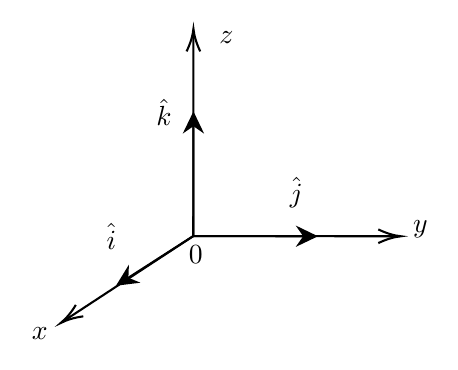
\begin{tikzpicture}[x=0.75pt,y=0.75pt,yscale=-1,xscale=1]
    %uncomment if require: \path (0,214); %set diagram left start at 0, and has height of 214
    
    %Straight Lines [id:da03185619981812238] 
    \draw    (339.92,139.91) -- (340.01,82.83) ;
    \draw [shift={(340.01,79.83)}, rotate = 90.09] [fill={rgb, 255:red, 0; green, 0; blue, 0 }  ][line width=0.08]  [draw opacity=0] (10.72,-5.15) -- (0,0) -- (10.72,5.15) -- (7.12,0) -- cycle    ;
    %Straight Lines [id:da9560574911529023] 
    \draw    (339.92,139.91) -- (397,140) ;
    \draw [shift={(400,140)}, rotate = 180.09] [fill={rgb, 255:red, 0; green, 0; blue, 0 }  ][line width=0.08]  [draw opacity=0] (10.72,-5.15) -- (0,0) -- (10.72,5.15) -- (7.12,0) -- cycle    ;
    %Straight Lines [id:da6801862667005925] 
    \draw    (339.92,139.91) -- (305.19,162.21) ;
    \draw [shift={(302.67,163.83)}, rotate = 327.29] [fill={rgb, 255:red, 0; green, 0; blue, 0 }  ][line width=0.08]  [draw opacity=0] (10.72,-5.15) -- (0,0) -- (10.72,5.15) -- (7.12,0) -- cycle    ;
    %Straight Lines [id:da9181595677149292] 
    \draw    (339.92,139.91) -- (438,140) ;
    \draw [shift={(440,140)}, rotate = 180.05] [color={rgb, 255:red, 0; green, 0; blue, 0 }  ][line width=0.75]    (10.93,-3.29) .. controls (6.95,-1.4) and (3.31,-0.3) .. (0,0) .. controls (3.31,0.3) and (6.95,1.4) .. (10.93,3.29)   ;
    %Straight Lines [id:da809113805207923] 
    \draw    (339.92,139.91) -- (340,42) ;
    \draw [shift={(340,40)}, rotate = 90.05] [color={rgb, 255:red, 0; green, 0; blue, 0 }  ][line width=0.75]    (10.93,-3.29) .. controls (6.95,-1.4) and (3.31,-0.3) .. (0,0) .. controls (3.31,0.3) and (6.95,1.4) .. (10.93,3.29)   ;
    %Straight Lines [id:da7519515623887656] 
    \draw    (339.92,139.91) -- (277.67,180.72) ;
    \draw [shift={(276,181.82)}, rotate = 326.75] [color={rgb, 255:red, 0; green, 0; blue, 0 }  ][line width=0.75]    (10.93,-3.29) .. controls (6.95,-1.4) and (3.31,-0.3) .. (0,0) .. controls (3.31,0.3) and (6.95,1.4) .. (10.93,3.29)   ;
    
    % Text Node
    \draw (385,110) node [anchor=north west][inner sep=0.75pt]    {$\hat{j}$};
    % Text Node
    \draw (320.64,72.4) node [anchor=north west][inner sep=0.75pt]    {$\hat{k}$};
    % Text Node
    \draw (296.64,132.4) node [anchor=north west][inner sep=0.75pt]    {$\hat{i}$};
    % Text Node
    \draw (336.36,142.8) node [anchor=north west][inner sep=0.75pt]    {$0$};
    % Text Node
    \draw (260.64,182.4) node [anchor=north west][inner sep=0.75pt]    {$x$};
    % Text Node
    \draw (444.33,131.13) node [anchor=north west][inner sep=0.75pt]    {$y$};
    % Text Node
    \draw (351,40) node [anchor=north west][inner sep=0.75pt]    {$z$};
    
    \end{tikzpicture}

\end{center}
    
    A partir do comum sistema de coordenadas acima, $\R^3$, temos que $\hat{i}$, $\hat{j}$ e $\hat{k}$ são vetores unitários, valendo a igualdade de seus módulos: $$\modvu{i}=\modvu{j}=\modvu{k}=1$$
    
    Se tomarmos um ponto $V$ qualquer, podemos escrevê-lo a partir dos vetores unitários $\hat{i}$, $\hat{j}$ e $\hat{k}$.
    
    \begin{center}

    \tikzset{every picture/.style={line width=0.75pt}} %set default line width to 0.75pt        
    
    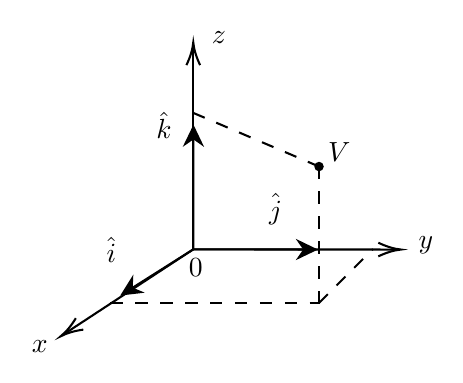
\begin{tikzpicture}[x=0.75pt,y=0.75pt,yscale=-1,xscale=1]
    %uncomment if require: \path (0,214); %set diagram left start at 0, and has height of 214
    
    %Straight Lines [id:da34741946249595057] 
    \draw    (339.92,139.91) -- (340.01,82.83) ;
    \draw [shift={(340.01,79.83)}, rotate = 90.09] [fill={rgb, 255:red, 0; green, 0; blue, 0 }  ][line width=0.08]  [draw opacity=0] (10.72,-5.15) -- (0,0) -- (10.72,5.15) -- (7.12,0) -- cycle    ;
    %Straight Lines [id:da35183475808822884] 
    \draw    (339.92,139.91) -- (397,140) ;
    \draw [shift={(400,140)}, rotate = 180.09] [fill={rgb, 255:red, 0; green, 0; blue, 0 }  ][line width=0.08]  [draw opacity=0] (10.72,-5.15) -- (0,0) -- (10.72,5.15) -- (7.12,0) -- cycle    ;
    %Straight Lines [id:da3444772189505243] 
    \draw    (339.92,139.91) -- (307.26,160.56) ;
    \draw [shift={(304.73,162.16)}, rotate = 327.69] [fill={rgb, 255:red, 0; green, 0; blue, 0 }  ][line width=0.08]  [draw opacity=0] (10.72,-5.15) -- (0,0) -- (10.72,5.15) -- (7.12,0) -- cycle    ;
    %Straight Lines [id:da5975516204182194] 
    \draw    (339.92,139.91) -- (438,140) ;
    \draw [shift={(440,140)}, rotate = 180.05] [color={rgb, 255:red, 0; green, 0; blue, 0 }  ][line width=0.75]    (10.93,-3.29) .. controls (6.95,-1.4) and (3.31,-0.3) .. (0,0) .. controls (3.31,0.3) and (6.95,1.4) .. (10.93,3.29)   ;
    %Straight Lines [id:da30250870787182804] 
    \draw    (339.92,139.91) -- (339.92,42.2) ;
    \draw [shift={(339.92,40.2)}, rotate = 90] [color={rgb, 255:red, 0; green, 0; blue, 0 }  ][line width=0.75]    (10.93,-3.29) .. controls (6.95,-1.4) and (3.31,-0.3) .. (0,0) .. controls (3.31,0.3) and (6.95,1.4) .. (10.93,3.29)   ;
    %Straight Lines [id:da12041369995991924] 
    \draw    (339.92,139.91) -- (277.67,180.72) ;
    \draw [shift={(276,181.82)}, rotate = 326.75] [color={rgb, 255:red, 0; green, 0; blue, 0 }  ][line width=0.75]    (10.93,-3.29) .. controls (6.95,-1.4) and (3.31,-0.3) .. (0,0) .. controls (3.31,0.3) and (6.95,1.4) .. (10.93,3.29)   ;
    %Shape: Circle [id:dp10671391488934368] 
    \draw  [fill={rgb, 255:red, 0; green, 0; blue, 0 }  ,fill opacity=1 ] (398.75,100) .. controls (398.75,99.03) and (399.53,98.25) .. (400.5,98.25) .. controls (401.47,98.25) and (402.25,99.03) .. (402.25,100) .. controls (402.25,100.97) and (401.47,101.75) .. (400.5,101.75) .. controls (399.53,101.75) and (398.75,100.97) .. (398.75,100) -- cycle ;
    %Straight Lines [id:da8040052427893101] 
    \draw  [dash pattern={on 4.5pt off 4.5pt}]  (400.5,100) -- (400.5,170.75) ;
    %Straight Lines [id:da4998664678624216] 
    \draw  [dash pattern={on 4.5pt off 4.5pt}]  (300,165.75) -- (400.5,165.75) ;
    %Straight Lines [id:da42817316260732885] 
    \draw  [dash pattern={on 4.5pt off 4.5pt}]  (400.5,165.75) -- (426.5,139.75) ;
    %Straight Lines [id:da5278231205946351] 
    \draw  [dash pattern={on 4.5pt off 4.5pt}]  (339.92,74.16) -- (400.5,100) ;
    
    % Text Node
    \draw (375,111.6) node [anchor=north west][inner sep=0.75pt]    {$\hat{j}$};
    % Text Node
    \draw (320.64,72.4) node [anchor=north west][inner sep=0.75pt]    {$\hat{k}$};
    % Text Node
    \draw (296.64,132.4) node [anchor=north west][inner sep=0.75pt]    {$\hat{i}$};
    % Text Node
    \draw (336.36,142.8) node [anchor=north west][inner sep=0.75pt]    {$0$};
    % Text Node
    \draw (260.64,182.4) node [anchor=north west][inner sep=0.75pt]    {$x$};
    % Text Node
    \draw (447,132.4) node [anchor=north west][inner sep=0.75pt]    {$y$};
    % Text Node
    \draw (347.44,33.6) node [anchor=north west][inner sep=0.75pt]    {$z$};
    % Text Node
    \draw (403.4,86.8) node [anchor=north west][inner sep=0.75pt]    {$V$};
    
    \end{tikzpicture}

\end{center}
    \[\overline{0V}=a\hat{i}+b\hat{j}+c\hat{k},\quad\text{$\forall$ $a$, $b$ e $c$ $\in$ $\R$}\]
    
    Para fins de notação, substituiremos $\hat{i}$ por $\undertilde{e_1}$, $\hat{j}$ por $\undertilde{e_2}$ e $\hat{k}$ por $\undertilde{e_3}$. De forma similar, substituiremos $x$ por $x_1$, $y$ por $x_2$ e $z$ por $x_3$. Assim, podemos reescrever o vetor $\overline{0V}$ como
    \[\underline{x}=x_1\undertilde{e_1}+x_2\undertilde{e_2}+x_3\undertilde{e_3}\]
    \begin{equation}
        \label{eqn:notacao_utilizada_01}
        \underline{x}=\sum_{i=1}^3x_i\undertilde{e_i}
    \end{equation}

    \subsection{Convenção indicial}
    
    Verificaremos formas mais compactas de se escrever um sistema de equações lineares. Por exemplo, o sistema abaixo
    \[
        \begin{cases}
            a_{11}x_1+a_{12}x_2+a_{13}x_3=b_1\\
            a_{21}x_1+a_{22}x_2+a_{23}x_3=b_2\\
            a_{31}x_1+a_{32}x_2+a_{33}x_3=b_3
        \end{cases}
    \]
    
    Advém do produto entre uma matriz $A$ com um vetor $\underline{x}$, da forma
    \[
        \underbrace{
            \begin{bmatrix} 
            	a_{11} & a_{12} & a_{13} \\
            	a_{21} & a_{22} & a_{23} \\
            	a_{31} & a_{32} & a_{33}
    	    \end{bmatrix}
    	}_{\displaystyle A}
    	\underbrace{
        	\begin{Bmatrix} 
                x_1 \\ x_2 \\ x_3
            \end{Bmatrix}
        }_{\displaystyle\underline{x}}
        =
        \underbrace{
            \begin{Bmatrix} 
                b_1 \\ b_2 \\ b_3
            \end{Bmatrix}
        }_{\displaystyle\underline{b}}
    \]
    
    Entretanto, ambas as formas acima podem ser reescritas de uma forma mais compacta, assim
    \[a_{i1}x_1+a_{i2}x_2+a_{i3}x_3=b_i\text{, para $i=1$, $2$ e $3$}\]
    
    Acima, o índice $i$ representa o \textbf{número de equações}. Podemos simplificar ainda mais introduzindo um somatório no índice restante
    \[\sum_{j=1}^3a_{ij}x_j=b_i\text{, para $i=1$, $2$ e $3$}\]
    
    A notação de Einstein remove o somatório acima, atribuindo um tipo para os índices conforme a quantidade de aparições que ele possui em um termo, sendo
    \[a_{ij}x_j=b_i\]
    \[
        \begin{cases}
            i=\text{ índice livre}\\
            j=\text{ índice mudo (somatório)}
        \end{cases}
    \]
    
    Como o índice $i$ apareceu apenas uma vez, ele é chamado de índice livre. Já o índice $j$ é chamado de índice mudo, representando implicitamente um somatório.
    
    Assim, podemos também reescrever de uma forma muito mais compacta a Equação (\ref{eqn:notacao_utilizada_01}) a partir da notação de Einstein, sendo
    \[\underline{x}=\sum_{i=1}^3x_i\undertilde{e_i}=x_i\undertilde{e_i}\]
    
    Por exemplo, como poderíamos simplificar um somatório duplo como o abaixo?
    \[\sum_{i=1}^3\sum_{j=1}^3a_{ij}b_{ij}\]
    
    Como os índices $i$ e $j$ se repetem duas vezes cada no mesmo termo, eles são índices mudos e indicam um somatório. Podemos reescrevê-los com a notação indicial de Einstein sem perda de significado:
    \[a_{ij}b_{ij}\]
    
    Expandindo o somatório acima,
    \[
        \displaystyle\overbrace{\displaystyle\underbrace{a_{11}b_{11}+a_{12}b_{12}+a_{13}b_{13}}_{\ShiftDown{0.5ex}{j=1\text{, }2\text{ e }3}}}^{\ShiftUp{0.5ex}{i=1}}+
        \displaystyle\overbrace{\displaystyle\underbrace{a_{21}b_{21}+a_{22}b_{22}+a_{23}b_{23}}_{\ShiftDown{0.5ex}{j=1\text{, }2\text{ e }3}}}^{\ShiftUp{0.5ex}{i=2}}+
        \displaystyle\overbrace{\displaystyle\underbrace{a_{31}b_{31}+a_{32}b_{32}+a_{33}b_{33}}_{\ShiftDown{0.5ex}{j=1\text{, }2\text{ e }3}}}^{\ShiftUp{0.5ex}{i=3}}
    \]